\documentclass[11pt]{article}
\usepackage{geometry}                % See geometry.pdf to learn the layout options. There are lots.
\geometry{a4paper}                   % ... or a4paper or a5paper or ... 
%\geometry{landscape}                % Activate for for rotated page geometry
%\usepackage[parfill]{parskip}    % Activate to begin paragraphs with an empty line rather than an indent
\usepackage{graphicx}
\usepackage{amssymb}
\usepackage{epstopdf}
\DeclareGraphicsRule{.tif}{png}{.png}{`convert #1 `dirname #1`/`basename #1 .tif`.png}

\usepackage{hyperref}
\usepackage{textcomp}
\usepackage[svgnames]{xcolor}
\usepackage{underscore}
\usepackage{parskip}
\usepackage[nosolutionfiles]{answers}
\usepackage{listings}

\newcommand{\normaltilde}{{\raise.17ex\hbox{$\scriptstyle\mathtt{\sim}$}}}
\newcommand{\unixcl}[1]{\texttt{\fcolorbox{black}{gray!20}{#1}}}

\Newassociation{sol}{Solution}{ans}
\newtheorem{ex}{Question}

\lstset{% general command to set parameter(s)
	basicstyle=\small\ttfamily,
    frame=single,
    numbers=left,
    xleftmargin=18pt,
    xrightmargin=4pt,
    fillcolor=\color{LightCyan!30},
    backgroundcolor=\color{LightCyan!30}
}

\lstdefinelanguage{OIL}
{
  morekeywords= {
	  RESOURCE, RESOURCEPROPERTY, STANDARD, INTERNAL, LINKED, LINKEDRESOURCE,
	  TASK, SCHEDULE, FULL, NONE, PRIORITY, EVENT, ISR, CATEGORY, OS, CPU, MEMMAP,
	  COMPILER, LINKER, SCRIPT, IOC, DATATYPENAME, DATATYPEPROPERTY, RECEIVER, SENDER, RCV_OSAPPLICATION, 	  RECEIVER_PULL_CB, ACTION, SENDER_ID, SND_OSAPPLICATION
	}
}

\lstset{
  language=OIL,
%  emph={
%    var,
%    expression,
%    string,
%    instruction_list,
%    template_file_name,
%    reader,
%    hierarchy
%  },
  emphstyle=\em,
  moredelim=[s]{"}{"},
  basicstyle=\ttfamily\small}


\newcommand{\LEDorange}{\textcolor{orange}{LED3}}
\newcommand{\LEDgreen}{\textcolor{LimeGreen}{LED4}}
\newcommand{\LEDred}{\textcolor{red}{LED5}}
\newcommand{\LEDblue}{\textcolor{blue}{LED6}}

\title{Trampoline Training\\$\star$\\\href{https://creativecommons.org/licenses/by-sa/3.0/fr/}{\small CC BY-SA 3.0}\\\vspace{5mm}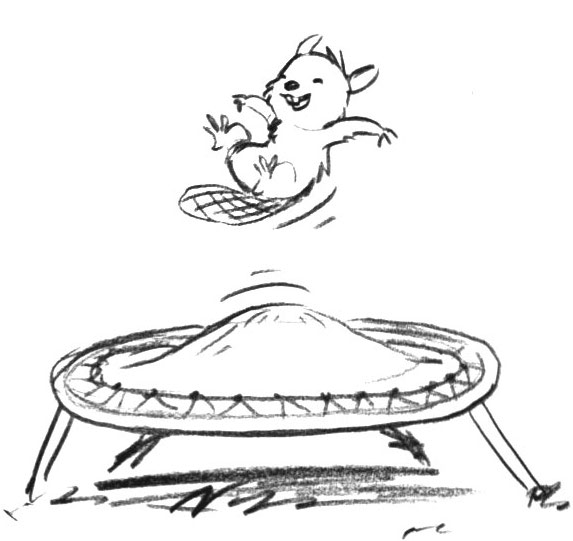
\includegraphics[width=2in]{Trampoline_Beaver_by_FancyFerret.jpg}\footnote{test}}
\author{}
%\date{}                                           % Activate to display a given date or no date

\begin{document}

\maketitle

{\bf Note:} All the software and documents are stored at \url{http://www.irccyn.ec-nantes.fr/~bechenne/trampoline}

\section{Goal}

The goal of this training is to become familiar with OSEK/VDX applications development process and with Trampoline. Trampoline is a Free Software implementation of the OSEK/VDX specification. Trampoline includes an OIL compiler which allows, starting from an OIL description, to generate OS level data structures of the application. In addition to the OIL description, the developer must provide the C sources of tasks and ISRs of the application. Trampoline runs on many  hardware platforms and we will use it on the Cortex-M4 STM32F4 Discovery board. If you have not installed Trampoline yet, get the Trampoline Package and read the install document.

The source code is located in the \unixcl{labs/labs_stm32F4_discovery} directory.

\section{The board}

We are going to use a demo board made by ST, the STM32F4 Discovery, with a Cortex M4 STM32F407 micro-controller. Here is a picture of the demo board:

\begin{center}
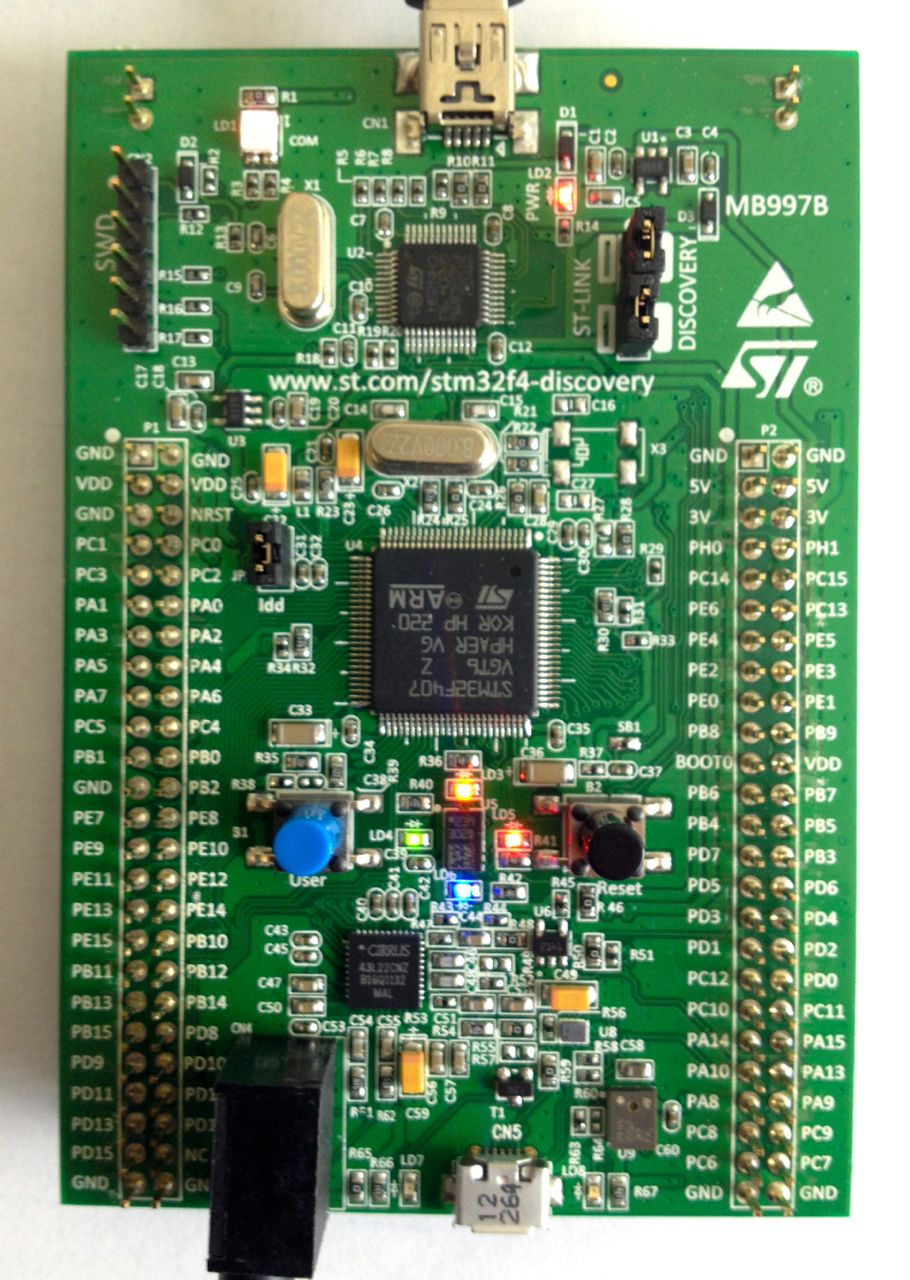
\includegraphics[width=.8\textwidth]{discovery.jpg} 
\end{center}

There are 4 LEDs located below the micro-controller. \LEDorange\ is the \textcolor{orange}{orange} one,  \LEDgreen\  is the \textcolor{LimeGreen}{green} one, \LEDred\ is the \textcolor{red}{red} one and \LEDblue\ is the \textcolor{blue}{blue} one. 

On the left, there is a \fcolorbox{blue}{LightSkyBlue}{blue button} labelled \texttt{User} that can be used for user interaction. On the right, there is a \fcolorbox{black}{black!20}{black button} which is the reset button.

The LEDs and the blue button are connected to the GPIO of the micro-controller. The GPIO is initialized with the LEDs as output and the button as input. The input corresponding to the button may be configured as an external interrupt line. The initialization is done by calling the \lstinline{initBoard} function. The argument of this function may be \lstinline{BUTTON_NOIT} to configure the corresponding GPIO input as a normal input or  \lstinline{BUTTON_IT} to configure the input as an external interrupt line. In summary \lstinline{initBoard(BUTTON_NOIT);} or \lstinline{initBoard(BUTTON_IT);} should be put in the \lstinline{main} function before starting Trampoline as shown below:

\begin{lstlisting}
FUNC(int, OS_APPL_CODE) main(void)
{
  initBoard(BUTTON_NOIT);
  StartOS(OSDEFAULTAPPMODE);
  return 0;
}
\end{lstlisting}

For the labs, functions are provided to switch on, switch off and toggle the LEDs. The unique argument is the LED identifier and should be \LEDorange, \LEDgreen, \LEDred\ or \LEDblue:

\unixcl{void ledOn(<led>)} turns on LED \lstinline{<led>}.\\
\unixcl{void ledOff(<led>)} turns off LED \lstinline{<led>}.\\
\unixcl{void ledToggle(<led>)} toggles LED \lstinline{<led>}.

A function gives the state of the  \texttt{User} blue button. It returns \lstinline{BUTTON_PRESSED} if the button is pressed and \lstinline{BUTTON_RELEASED} if not.

\unixcl{ButtonState readButton();} returns the state of the \texttt{User} blue button. 

At last a function called \lstinline{delay} waits for an amount of time expressed in milliseconds.

\unixcl{void delay(<howManyMs>);} waits \lstinline{<howManyMs>} ms. 

Will will use this function to slow down the application.

\subsection{A word about memory sections}

AUTOSAR defines a way to put objects: constants, variables and functions in memory sections in a portable way\footnote{memory section declaration is not part of the C standard}. For that, a set of macro are used along with a generated file : MemMap.h. Functions should be declared with the \lstinline{FUNC} macro, variables with the \lstinline{VAR} macro, constants with the \lstinline{CONST} macro and pointers to variables, pointers to constant, constant pointers to variable and constant pointers to constant with \lstinline{P2VAR}, \lstinline{P2CONST}, \lstinline{CONSTP2VAR} and \lstinline{CONSTP2CONST} respectively. Sections are opened and close with a macro definition and the inclusion of the \lstinline{tpl_memmap.h} file. For instance:

\begin{lstlisting}
#define APP_Task_my_periodic_task_START_SEC_VAR_32BIT
#include "tpl_memmap.h"
VAR(int, AUTOMATIC) period;
VAR(int, AUTOMATIC) occurence;
#define APP_Task_my_periodic_task_STOP_SEC_VAR_32BIT
#include "tpl_memmap.h"
\end{lstlisting}

defines variables \lstinline{period} and \lstinline{occurence} in the variables section of task \lstinline{my_periodic_task}.

\begin{lstlisting}
#define APP_Task_my_periodic_task_START_SEC_CODE
#include "tpl_memmap.h"
TASK(my_periodic_task)
{
  ...
  TerminateTask();
}
#define APP_Task_my_periodic_task_STOP_SEC_CODE
#include "tpl_memmap.h"
\end{lstlisting}

defines the task \lstinline{my_periodic_task} in the code section of task \lstinline{my_periodic_task}. \lstinline{goil} generates the sections for tasks according to the description.

\section{Basic tasks}

Go into the lab1 directory. There are 2 files:

\begin{description}
\item[lab1.oil] the OIL description of the lab1 application;
\item[lab1.c] the C source for the lab1 task.
\end{description}

Edit the lab1.oil and look at the \texttt{TRAMPOLINE_BASE_PATH} attribute (in OS $>$ BUILD attribute).  \texttt{TRAMPOLINE_BASE_PATH} is set to \texttt{"../../.."}. If you move around the lab1 directory you will have to update this attribute.

lab1 is a very simple application with only 1 task called \lstinline{a_task}. \lstinline{a_task} starts automatically (\texttt{AUTOSTART = TRUE} in the OIL file). Look at the OIL file and the C source file.

To compile this application, go into the lab1 directory and type:\\
\unixcl{goil -t=thumb2/cortex-m4/STM32F4-Discovery lab1.oil}

%Goil templates are located in \texttt{trampoline/goilv2/templates}.
\texttt{goil} is the OIL compiler. It parses the OIL file and produces a set of C files. The \texttt{-t} option gives the target system. \texttt{thumb2} is the instruction set of the target, \texttt{cortex-m4} is the micro-controller core and \texttt{STM32F4-Discovery} is the board.\\\texttt{thumb2/cortex-m4/STM32F4-Discovery} is a path inside the \texttt{machines} directory and in the \texttt{templates} directory. The OIL file gives the names of the C source files (with \texttt{APP_SRC} and the name of the executable file (with \texttt{APP_NAME}).

This generate a Makefile for the application too. It has to be done only once. If you change something in the OIL file or in your C file, you do not need to rerun the goil compiler by hand because make will run it when needed. Then type:

\unixcl{make}

The application and Trampoline OS are compiled and linked together. To load the application on the target, type:

\unixcl{make burn}

The application may or may not start :-). Press the reset button if it does not start.

In this application, there is only one task called \lstinline{a_task} which switches \LEDorange\ on.

\begin{lstlisting}
TASK(a_task)
{
  ledOn(LED3);
  TerminateTask();
}
\end{lstlisting}

\section{OS system calls and task launching}

\subsection{Task activation and scheduling}


The \texttt{ActivateTask()} system call allows to activate another task of the application.

Go into the \texttt{lab2} directory.

In \texttt{lab2.oil} and \texttt{lab2.c}, 2 tasks have been added: \texttt{task_0} (priority 1) and \texttt{task_1} (priority 8). \texttt{task_0} toggles \LEDgreen\ on and \texttt{task_1} toggles \LEDred\ on. Task \texttt{a_task} activates \texttt{task_0} and \texttt{task_1}. All statements are separated by a busy-wait loop on the button so that by pressing the button we can control the execution. Examine the OIL and the C files.

Compile and execute. Why does \texttt{task_1} execute before \texttt{task_0} whereas it has been activated after?

\subsection{Task chaining}

The \texttt{ChainTask()} system call allows to chain the execution of a task to another one. This is roughly the same thing as calling ActivateTask and TerminateTask at the same time.

Replace the call to \texttt{TerminateTask} by a \texttt{ChainTask(task_1)} at the end of task \texttt{a_task}. What is happening?

Chain to \texttt{task_0} instead of \texttt{task_1}. What is happening?

Test the error code returned by \texttt{ChainTask} and correct your program to
handle the error. \texttt{ChainTask} may return the following codes:

\begin{description}
\item[E_OS_ID] the target task does not exist;
\item[E_OS_RESOURCE] the calling task holds a resource;
\item[E_OS_CALLEVEL] not called from a task;
\item[E_OS_LIMIT] too many activations of the target task.
\end{description}

\subsection{Pre-task and Post-task hooks}

Hook routines are used to insert application functions inside the kernel. Hook routines are called by the kernel when a particular event happens. The Pre-task hook is called when a task goes into the running state. The Post-task hook is called when a task leaves the running state. Hooks are useful for debugging purpose.

There are two boolean attributes in the OS object of the OIL to use Pre-task and Post-task hooks:

\begin{lstlisting}[language=OIL]
  OS config {
    STATUS = EXTENDED;
    PRETASKHOOK = TRUE;
    POSTTASKHOOK = TRUE;
    
  ...
\end{lstlisting}

When these hooks are used, the user have to write a hook functions:

\begin{lstlisting}
FUNC(void, OS_CODE) PreTaskHook()
{
  ...
}
\end{lstlisting}

for the pre-task hook and

\begin{lstlisting}
FUNC(void, OS_CODE) PostTaskHook()
{
  ...
}
\end{lstlisting}


Go into the \texttt{lab3} directory and play with the application which is in it. It is the same application as in \lstinline{lab2} with the use of \lstinline{delay} instead of busy-wait for the blue button. Pre and post task hooks are used to switch a led corresponding to the running task on.

\subsection{Extended tasks and synchronization using events}

Go into the \lstinline{lab4} directory.

This application has 2 tasks : \lstinline{a_task} which is an extended task and \lstinline{task_0} which is a basic task. En extended task has at least one event declared in the OIL file.

Look at the OIL file and at the C file. The application does not work as expected. What is happening ? Correct the OIL file to have a proper behavior.


Unlike a basic task, an extended task may wait for an event. In the OIL file, set the priority of \texttt{task_0} to 8 and add 2 events \texttt{evt_0} and \texttt{evt_1}. \texttt{evt_0} is used by \texttt{task_0} and \texttt{evt_1} is used by \texttt{task_1}. \texttt{a_task} activates \texttt{task_0} and \texttt{task_1} then sets \texttt{evt_0} and \texttt{evt_1} and terminates. \texttt{task_0} and \texttt{task_1} wait for their event, clear it and terminate.




\begin{ex}
Write the corresponding application. Compile and execute the application. What is happening?
\end{ex}

\begin{ex}
Program an application conforming to the following requirements: The application has 2 tasks:
\texttt{server} priority 2, \texttt{t1} priority 1.

server is an infinite loop that activates \texttt{t1} and waits for event \texttt{evt_1}. \texttt{t1} prints ``I am t1'' and sets \texttt{evt_1} of \texttt{server}. Explain how it works.
\end{ex}

\begin{ex}
Extend the previous application by adding 2 tasks: \texttt{t2} and \texttt{t3} (priority 1 for both) and 2 events \texttt{evt_2} and \texttt{evt_3}. \texttt{server} activates \texttt{t1}, \texttt{t2} and \texttt{t3} and waits for one of the events. When one of the events is set, \texttt{server} activates the corresponding task again.
\end{ex}

\begin{ex}
Try many priority combinations for the tasks. Explain the behavior.
\end{ex}
\end{document}  